    \begin{itemize}
    
    	\item \textbf{Librería Front-end:} Una librería Front-end \cite{frontEnd2}es una herramienta que es agregada a nuestros proyectos, en este caso Web, el cual incorpora elementos que otras personas o equipos ya desarrollaron, sumando funcionalidad a nuestra Web, reduce el mantenimiento y el tiempo de desarrollo, algunas características que existen actualmente y pueden agregarse van desde gráficas, animaciones, mapas etc. 
      
       \item \textbf{NPM :} NPM \cite{npm} es un gestor de paquetes que nos permite agregar dependencias a cualquier proyecto basado en Javascript, esto es posible con un cliente de líneas de comandos que es útil para poner o quitar los paquetes que deseamos. La configuración consta de un archivo en el cual contiene una lista de las dependencias que se quieren instalar en nuestro proyecto. Actualmente existen miles de paquetes que pueden ser descargados de manera gratuita y de igual manera permite colaborar. 
       
       \item \textbf{ React :} React \cite{react} es una librería de Javascript para el desarrollo de interfaces de usuario (Front-end), famosa por la posibilidad de hacer fácilmente Webs de usa sola página. React fue desarrollada por Facebook y con el paso del tiempo, conocidas empresas han empezado a implementarlo en sus proyectos. 
    React nos permite desarrollar de una forma más ordenada y con el menos código necesario. 
    Se considera que React no es un Framework en comparación con ANGULAR o EMBER porque no tiene cada una de las áreas que propone el modelo vista controlador, este solo se encarga de las vistas. 
    Uno de los puntos fuertes de React es que cuenta con un DOM virtual el cual es almacenado en memoria, esto provoca que cuando algo cambie este se va reflejado en memoria de una forma más rápida, después el DOM virtual será comparado con el DOM del navegador y solo actualizara lo que encuentre diferente. 
    React funciona en base a componentes que pueden ser reusados cuantas veces sea necesario, una forma fácil de entenderlo puede ser como la programación orientada a objetos al hacer una instancia de una clase, estos componentes pueden tener un estado, que es encapsulado por sí solo, de manera local por cada uno y puede ser actualizado.
    Los tres elementos principales de React son los siguientes:
 \begin{itemize}
 
 
 \item \textbf{Componente:}Una manera fácil de explicar un componente en React es compararlo con la programación orientada a objetos, en la cual un componente es un objeto, en el que este es una base ya establecida con propiedades. Si se instancian varios objetos de el mismo tipo, estos tendrán características en común pero con ciertas propiedades que los hacen distintos entre ellos. Con este principio podemos crear varios componentes en los cuales solo cambia algún elemento diferencial, como un texto una imagen etc.
  \item \textbf{Estado:}El estado en react siguiendo la analogía de la programación orientada a objetos, son los atributos de la clase, pero estos son internamente manejados por React, esto se refiere a que para actualizar el estado se debe usar una función proporcionada por la librería.
   \item \textbf{Props:}Los props son los parámetros  que se le da a nuestro componente para que este actúe de manera diferente a los otros componentes de el mismo tipo.
 \end{itemize}
 React crea un árbol en el cual hace una copia de el DOM que guarda en la memoria RAM, una de las principales ventajas de React es la que aquí se trata. Una vez el árbol creado, este espera a que alguno de los miembros del estado se actualice y actualiza el nodo que depende de ese estado. Con esto actualiza el DOM del navegador pero solo la parte diferencia, agilizando todo el proceso.

Por ejemplo si tenemos una lista nombres en nuestra Web y el usuario borra uno, el navegador quitará el elemento que el usuario elige, pero no se volverá a hacer el render de toda la Web.

Existen dos componentes dentro de React uno es el componente classe y otro el componente función, con los que se puede tener los mismos resultados pero se usan a criterio propio.

En la siguiente imagen se encuentra un componente tipo clase, en el cual nos sirve para hacer una calculadora que suma o resta un parámetro dado.
 \newline
       \begin{figure}[H]
       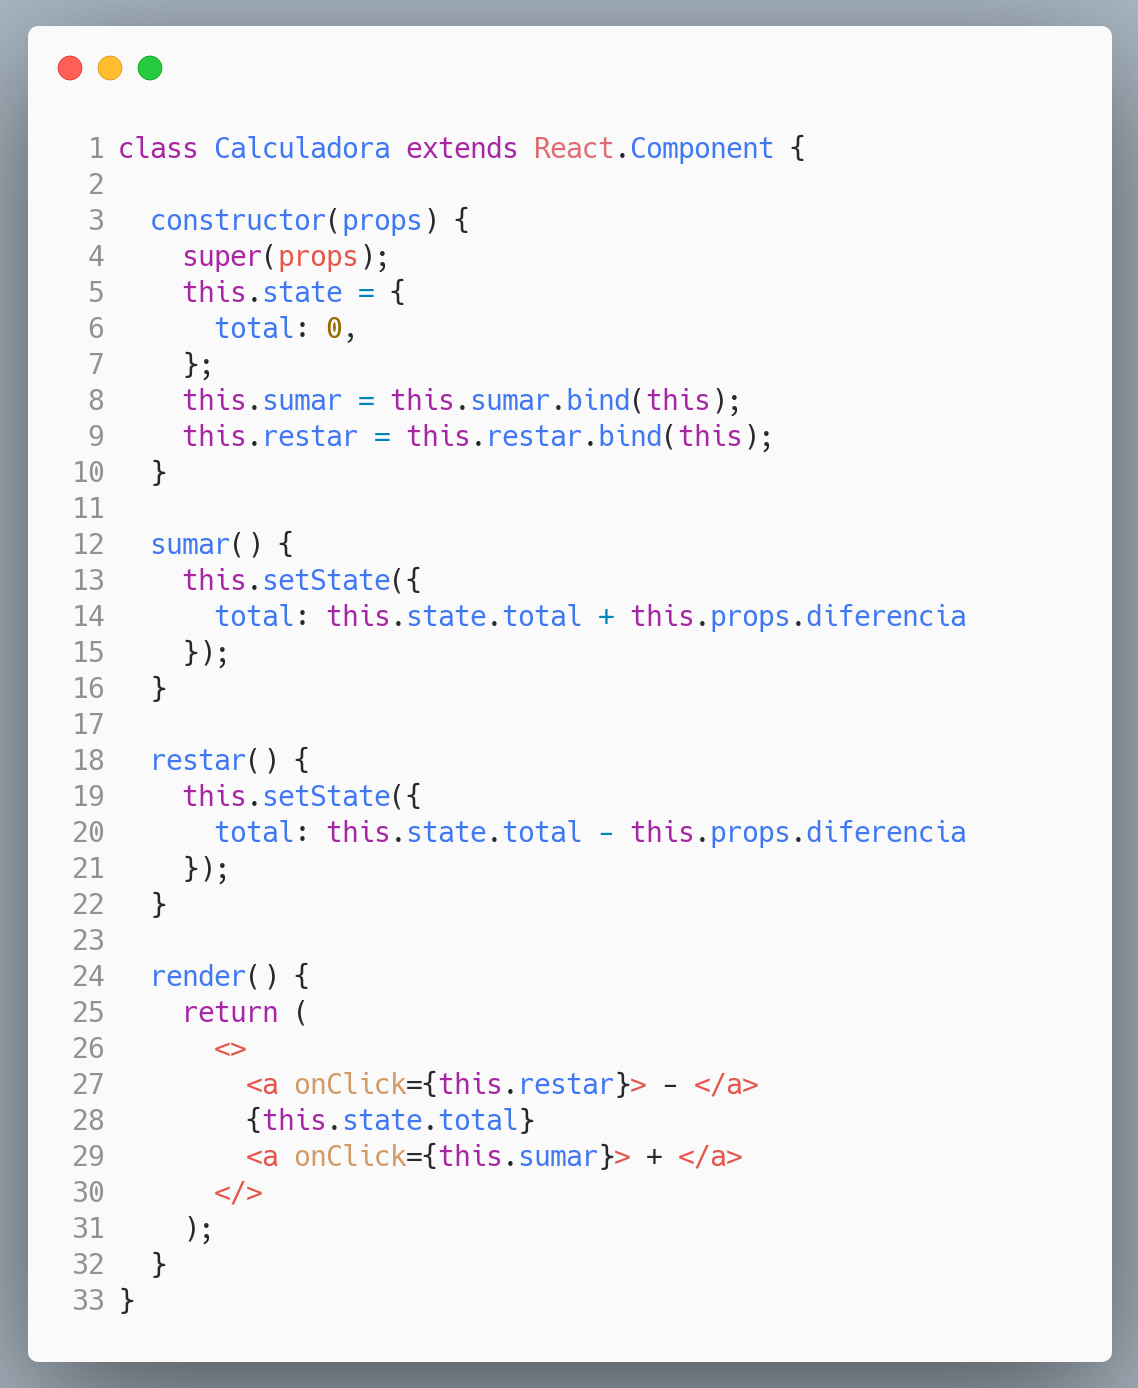
\includegraphics[width=1\textwidth]{./Imagenes/classe.png}
        \caption[Componente calculadora]{Componente calculadora}
       \end{figure}
       \newline
    En la línea 5 dentro del constructor se inicializa el estado de nuestro componente el cual guarda el total acumulado.

Dentro del return que está en el render tenemos dos etiquetas <a> ( Línea 27 y 29 ) las cuales son los botones de suma y resta de nuestra aplicación, estas hacen un llamado a las funciones de suma y resta dependiendo el operador.
En la línea 28 mostramos el total acumulado obteniendolo de el estado mediante this.state más el nombre del elemento del estado.

Las funciones sumar y restar actualizan el estado mediante this.setState, función que recibe un objeto con los datos de JavaScript que va a actualizar. En este caso suma o resta un parámetro dado por props. 

La forma de hacer el llamado a un componente es la siguiente. 
 \newline
       \begin{figure}[H]
       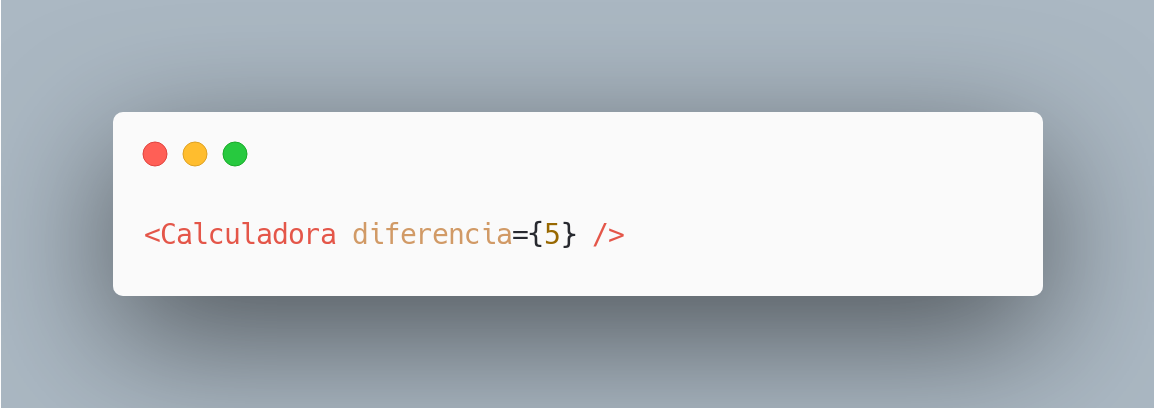
\includegraphics[width=1\textwidth]{./Imagenes/componente.png}
        \caption[Llamado a componente]{Llamado a componente}
       \end{figure}
       \newline
       \item \textbf{HTML  :}   HTML \cite{html} es un lenguaje con un conjunto de etiquetas que permite definir el contenido con el que podemos interactuar dentro de una página Web. 
       
       \item \textbf{ SASS :} SASS \cite{scss} es un preprocesador de CSS, el cual nos ayuda a agregar características que no tiene CSS puro y que son propias de los lenguajes de programación como variables, funciones, herencia entre otros. Nos permite dedicar menos tiempo para mantener y crear el CSS y agrega la posibilidad de tener una organización modular. 
       
       \item \textbf{ Webpack :} Hace algunos años Javascript iniciaba como un lenguaje que nos permitía agregar interacción a nuestras páginas Web, que anteriormente eran simplemente contenido estático.  Javascript nos permitía recuperar los datos que eran introducidos en formularios, podíamos mostrar ventanas emergentes o incluso agregar animaciones. Para agregar Javascript en nuestros archivos de HTML, se debía agregar la etiqueta <script>, donde se indicaba la ruta donde estaba almacenado nuestro archivo .js de Javascript.  
    Años más tarde se agregó soporte al lenguaje Javascript, para permitir hacer peticiones asíncronas a nuestros servidores, esto hizo que las empresas empezaran a ver como viable el desarrollo Web, que previamente estaba enfocado en el desarrollo de escritorio, también hizo que los archivos .js empezaran a crecer en cantidad de líneas en nuestros proyectos, y se miraba reflejado en nuestros archivos .HTML los cuales empezaron a tener múltiples etiquetas <script>. Lo que significaba múltiples peticiones para obtener los archivos del servidor, esto agregaba una capa de complejidad, debido a la inclusión de múltiples archivos .js embebidos en un .HTML y al agregarlos se debe tener en cuenta el orden en que se listan, porque es posible que tengan dependencias entre ellos. Actualmente es posible comprimir los múltiples archivos .js para que sean menos peticiones al servidor (CDN).  Cuando un proyecto con Javascript crecía aumentaba el número de módulos que se agregan, pero no existía la forma de gestionarlos. Un problema que tenía Javascript es que los navegadores no soportan un sistema nativo de módulos por eso se agregaron Require.js y Common JS. 
    En base a esto nació Webpack \cite{webPack} que permite usar NPM como gestor de dependencias y soporta el sistema de módulos Common JS.
    Webpack permite modular nuestro código, para esto genera un grafo dado un punto de entrada, el punto de entrada es el nodo inicial de nuestro grafo, el grafo es generado con las inclusiones de elementos encontrados en los archivos, como son imágenes, archivos de CSS etc. Esto genera un archivo final en el que estará el empaquetado de nuestros archivos. 
    Webpack nos permite especificar cargadores para distintos tipos de archivos como imágenes, SCSS, CSS, HTML. JSX, etc. ya que nativamente solo admite archivos Javascript. 
    La configuración es dada por un archivo que se coloca en la raíz del proyecto.
    
       \item \textbf{Babel  :}   Babel \cite{babel} es un traductor de código Javascript, que permite convertir el código Javascript más moderno en alguna versión más vieja, esto nos proporcionó la capacidad de que nuestro código pueda ser ejecutado por más cantidad de navegadores, los cuales solo pueden interpretar versiones anteriores de Javascript. Por ejemplo, el siguiente código es usado en React para mostrar un texto. 
    \begin{figure}[H]
    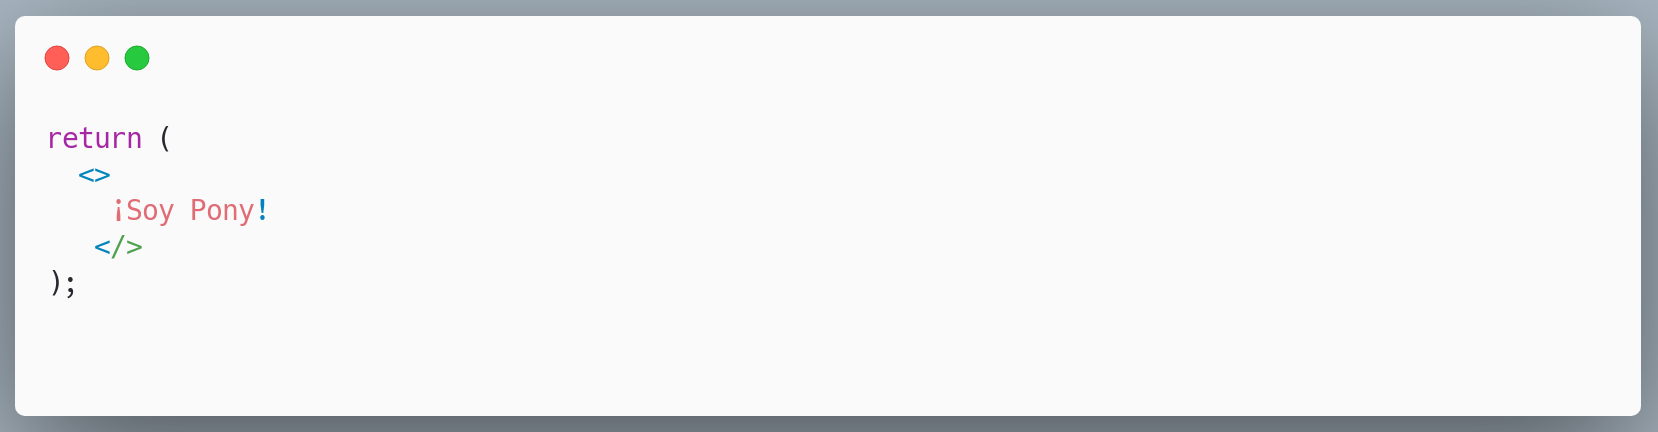
\includegraphics[width=1\textwidth]{./Imagenes/image16.png}
    \caption[Impresión de texto con React]{Impresión de texto con React}
    \end{figure}
       El código será convertido en el que se muestra En la figura 7.4, el cual es interpretada por un mayor número de navegadores. 
       \newline
       \newline
       \begin{figure}[H]
       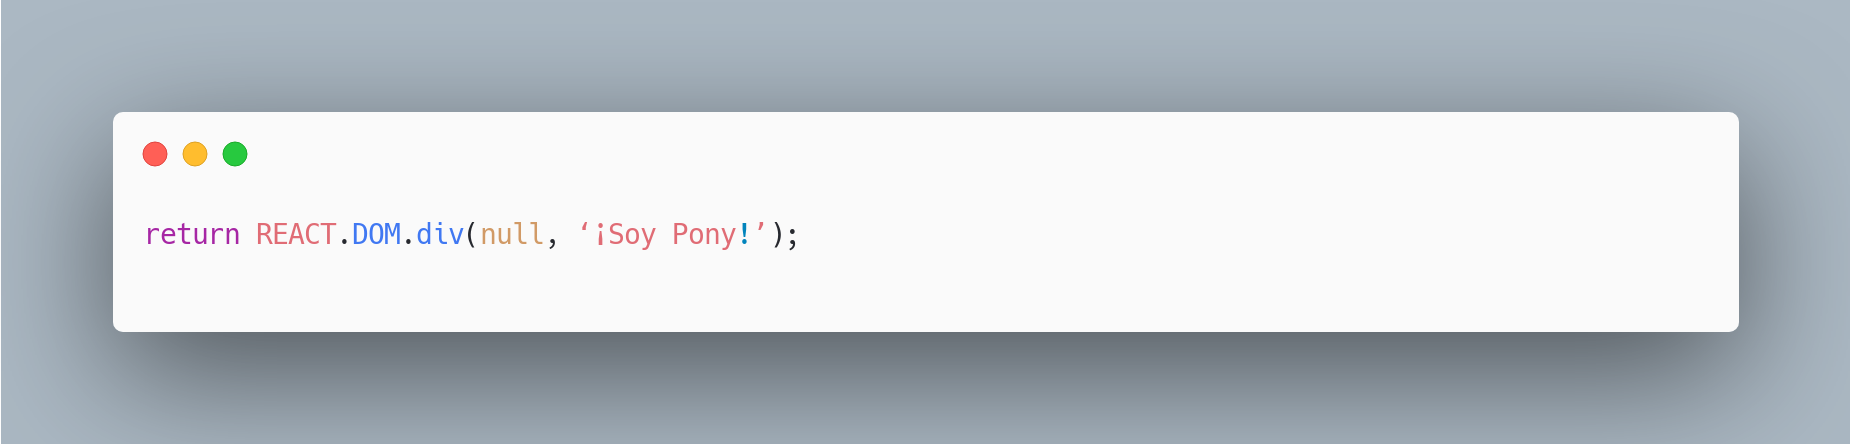
\includegraphics[width=1\textwidth]{./Imagenes/image5.png}
        \caption[Impresión de texto una vez el código es convertido]{Impresión de texto una vez el código es convertido}
       \end{figure}
       \newline
       \newline
       \item \textbf{ESLint :}ESLint nos permite definir una guía de estilos en nuestro código, lo que nos ayudará a tener un código limpio y claro para que sea fácil de editar y mantener, podemos agregar guías de estilos una de ellas es la de Airbnb, que es una de las más usadas. 
       
    \end{itemize}